%==============================================================================
\section{Solution de principe}
%==============================================================================

\begin{frame} \FT{Solutions}
    \BI
        \o Routage des interruptions $\rightarrow$ Composant IOPIC 
        \o Canaux de l'IOC $\rightarrow$ MULTI\_IOC 
    \EI
\end{frame} %-------------------------------------------------------------------

\begin{frame} \FT{Solution pour affichage des machines virtuelles - Lecture}
        \begin{center}
                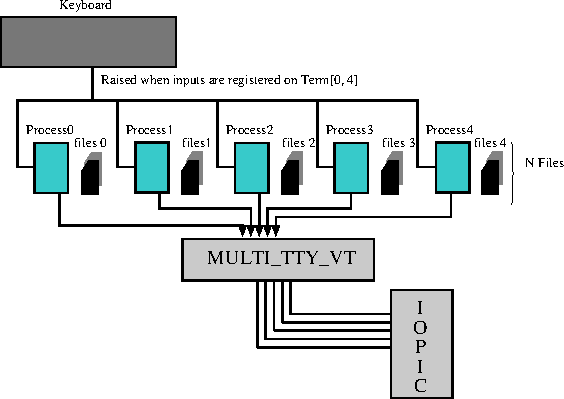
\includegraphics[width=10cm]{ttys_adv_r.pdf}
        \end{center}
        % Pour r�soudre le probl�me de l'affichage des instances d'ALMOS il est n�cessaire de cr�er un nouveau composant
        % � partir du composant MULTI\_TTY.
        % Le probl�me � r�soudre �tait de limiter le nombre de terminaux cr�es par la simulation.
        % Ce composant permet d'afficher sur un terminal, via une commande sur le terminal hyperviseur,
        % l'une ou l'autre des instances d'ALMOS.
        % Il y a donc un terminal pour l'hyperviseur et 4 terminaux pour toutes les instances d'ALMOS.
        % Cette commande doit int�ragir non seulement avec le MULTI_TTY_VT mais aussi avec le composant IOPIC.
        % En effet lorsque l'on bascule l'affichage d'une fen�tre, on souhaite aussi que les interruptions soit
        % redirig�s vers l'instance que l'on est en train d'afficher.
        % Il faut donc reconfigur� l'IOPIC pour qu'il envoie l'interruption � la bonne instance.
\end{frame}

\begin{frame} \FT{Solution pour affichage des machines virtuelles - �criture}
        \begin{center}
                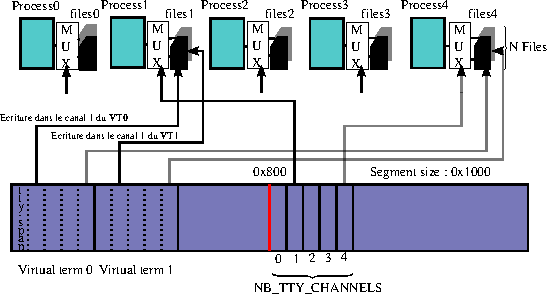
\includegraphics[width=10cm]{ttys_adv_w.pdf}
        \end{center}
\end{frame}

\begin{frame} \FT{Solution pour le d�marrage des machines virtuelles}
        \begin{center}
                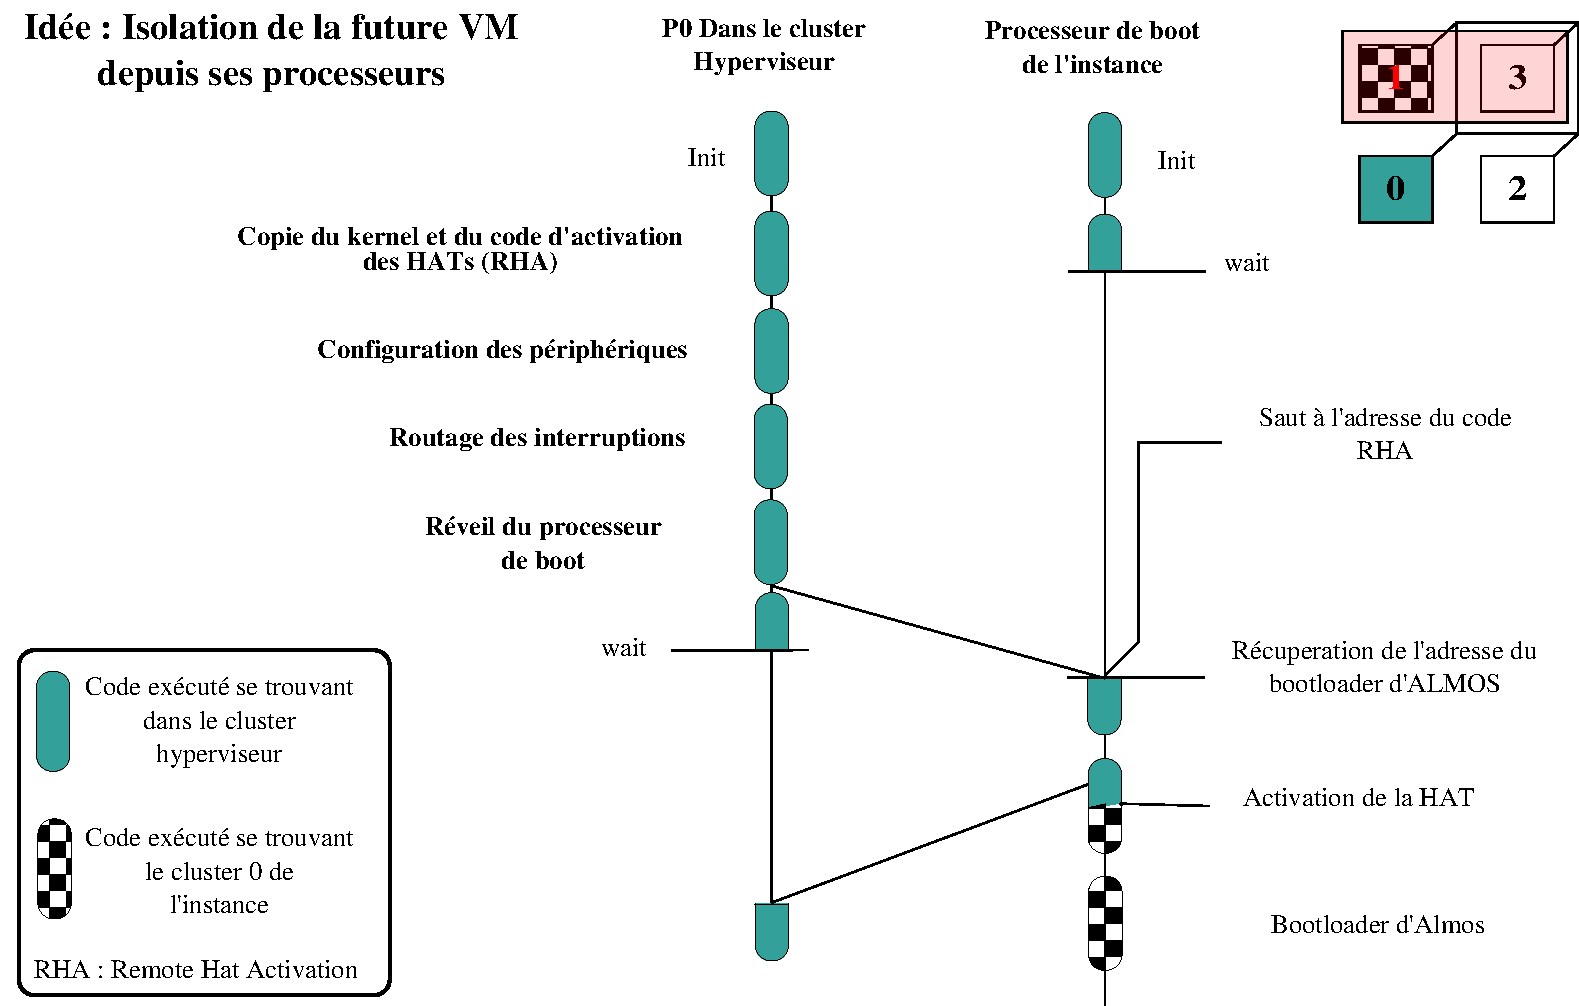
\includegraphics[width=12cm]{boot_simple.pdf}
        \end{center}
\end{frame}
